\documentclass[11pt]{amsart}
\usepackage{amsmath,amssymb,amsthm}
\usepackage[margin=1in]{geometry}
\usepackage{microtype}
\usepackage{tikz}
\usetikzlibrary{arrows.meta}
\usepackage{hyperref}

\theoremstyle{plain}
\newtheorem{thm}{Theorem}[section]
\newtheorem{lem}[thm]{Lemma}
\newtheorem{prop}[thm]{Proposition}
\newtheorem{cor}[thm]{Corollary}
\theoremstyle{definition}
\newtheorem{defn}[thm]{Definition}
\newtheorem{rem}[thm]{Remark}

\DeclareMathOperator{\conv}{conv}
\DeclareMathOperator{\Pol}{Pol}
\newcommand{\B}{\{0,1\}}
\newcommand{\med}{\mathrm{med}}

\title[The order-convex clone on the cube: unbounded width and NP-hardness]
{The order-convex clone on the Boolean cube: unbounded width,
 NP-hardness, and median-closure as the exact boundary}

\author{Ryota Shibusawa}
\address{Daiichi Institute of Technology, Japan}
\email{r-shibusawa@daiichi-koudai.ac.jp}

\subjclass[2020]{08A70, 68Q25; 08B05, 06D30, 55U35}
\keywords{constraint satisfaction, bounded width, Taylor polymorphism,
  Siggers operation, weak near-unanimity, order-convex set, distributive
  lattice, NP-completeness, cubical set}

\begin{document}

\begin{abstract}
  The realizability of a cell along a monotone generator of the cube
  category is a monotone-selection constraint problem whose variable
  domains are the fibres of the generator.  When those fibres are
  closed under the median the problem carries a majority polymorphism
  and hence has strict width two; the coskeletal dimension of the
  corresponding cubical atom is then bounded by the arity of the
  median rather than by the ambient dimension.  We show that this
  bound has an exact algebraic boundary.  Let $L_m$ be the relational
  structure on $\B^m$ whose relations are the order and all
  order-convex subsets.  We prove that for every $m\ge 3$ the clone
  $\Pol(L_m)$ contains \emph{no} ternary weak near-unanimity
  operation; consequently $L_m$ does not have bounded width.  The
  proof reduces to the single Boolean cube $\B^3$ by an order-convex
  restriction, where the absence is established by hand from a
  twelve-cell contradiction (a minimal core located by machine).  The
  same restriction, applied to the $4$-ary Siggers operation, shows the
  clone is not even Taylor, so the constraint problem is in fact
  $\mathrm{NP}$-complete for every $m\ge 3$ (and in $\mathrm P$ for
  $m\le 2$).  Thus median-closure of the fibres is precisely the
  boundary---between bounded width and unbounded width, and between
  polynomial-time and $\mathrm{NP}$-hard realizability---and a cubical
  atom with a non-median-closed generator is unboundedly coskeletal in
  every dimension.
\end{abstract}

\maketitle

\section{Introduction}

The Dedekind cube category $\square$ is the Lawvere theory of bounded
distributive lattices: its morphisms $[k]\to[m]$ are the monotone maps
$\B^k\to\B^m$.  A \emph{cell} of a presheaf is realizable along a
monotone generator $z\colon\B^m\to\B^n$ exactly when it factors through
$z$, and this factorization problem is, vertexwise, a
\emph{monotone-selection constraint satisfaction problem}: for a cell
$a\colon\B^k\to\B^n$ one seeks a monotone $g\colon\B^k\to\B^m$ with
$z\circ g=a$, i.e.\ one variable $g(v)$ per vertex $v$ of $\B^k$, with
domain the fibre $z^{-1}(a(v))$ and a binary constraint $g(v)\le g(v')$
along each edge $v\le v'$.  The companion work~\cite{PaperW} shows that
when every fibre $z^{-1}(q)$ is closed under the ternary median
$\med(x,y,z)=(x\wedge y)\vee(y\wedge z)\vee(z\wedge x)$, this constraint
problem carries the median as a \emph{majority polymorphism}, so by the
Baker--Pixley theorem~\cite{BakerPixley} it has \emph{strict width
two}: it is solvable if and only if it is $(2,3)$-consistent, and the
solution set is determined by its two-variable projections.  The
associated cubical atom is then determined by its cells of bounded
level---its coskeletal dimension is governed by the arity $3$ of the
median, not by the ambient dimension---so that such atoms are finite in
number.

The hypothesis that the fibres be median-closed is essential.  A fibre
of a monotone map is always \emph{order-convex} (if $a\le c\le b$ and
$z(a)=z(b)=q$ then $z(c)=q$), but need not be median-closed: the
antichain $\{001,010,100\}\subseteq\B^3$ has median $000$, which lies
below all three of its members (Figure~\ref{fig:cube}), so an
order-convex set containing the antichain but not $000$ is not
median-closed.  This note settles what happens for general order-convex
fibres.  The relevant object is the relational structure carrying
\emph{all} order-convex relations, and the question is whether it has
bounded width in the sense of Feder and Vardi.  We prove it does not, in
every dimension $m\ge 3$, and that the median-closed case is the exact
boundary.

\begin{figure}[ht]
\centering
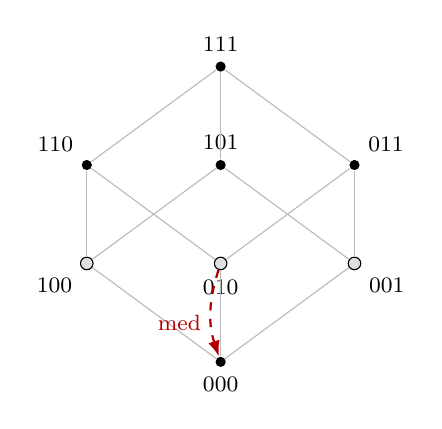
\begin{tikzpicture}[x=1.7cm,y=1.25cm,
    every node/.style={font=\footnotesize},
    dot/.style={circle,fill,inner sep=1.3pt},
    atom/.style={circle,draw,fill=black!12,inner sep=1.6pt}]
  \node[dot,label=below:$000$] (b) at (0,0) {};
  \node[atom,label=below left:$100$] (a1) at (-1,1) {};
  \node[atom,label=below:$010$] (a2) at (0,1) {};
  \node[atom,label=below right:$001$] (a3) at (1,1) {};
  \node[dot,label=above left:$110$] (c1) at (-1,2) {};
  \node[dot,label=above:$101$] (c2) at (0,2) {};
  \node[dot,label=above right:$011$] (c3) at (1,2) {};
  \node[dot,label=above:$111$] (t) at (0,3) {};
  \foreach \a/\c in {a1/c1,a1/c2,a2/c1,a2/c3,a3/c2,a3/c3}
     \draw[gray!55] (\a)--(\c);
  \foreach \a in {a1,a2,a3} \draw[gray!55] (b)--(\a);
  \foreach \c in {c1,c2,c3} \draw[gray!55] (\c)--(t);
  \draw[-{Latex[length=2mm]},red!70!black,thick,dashed]
     (a2) to[bend right=18] node[left,pos=0.62]{$\med$} (b);
\end{tikzpicture}
\caption{The cube $\B^3$.  The three atoms $100,010,001$ (shaded) form an
antichain whose convex hull is themselves; but their median is the
bottom $000$, which escapes the hull.  A ternary majority operation
compatible with all order-convex sets is thereby obstructed, and the
theorem shows no weak near-unanimity operation avoids the obstruction.}
\label{fig:cube}
\end{figure}

\section{The order-convex structure and its clone}

\begin{defn}
  For $m\ge 1$ let $\B^m$ carry the componentwise partial order.  A set
  $C\subseteq\B^m$ is \emph{order-convex} if $a,b\in C$ and $a\le c\le
  b$ imply $c\in C$.  Let $L_m$ be the relational structure on the
  domain $\B^m$ whose relations are the order
  $\le\;=\{(x,y):x\le y\}$ and every order-convex subset $C\subseteq
  \B^m$ regarded as a unary relation.
\end{defn}

An operation $f\colon(\B^m)^k\to\B^m$ is a \emph{polymorphism} of $L_m$
if it preserves every relation; we write $\Pol(L_m)$ for the clone of
all polymorphisms.  Preservation unwinds as follows.

\begin{lem}\label{lem:polchar}
  $f\in\Pol(L_m)$ if and only if $f$ is
  \begin{enumerate}
  \item \emph{monotone}: $x_i\le y_i$ for all $i$ implies
    $f(x_1,\dots,x_k)\le f(y_1,\dots,y_k)$;
  \item \emph{idempotent}: $f(x,\dots,x)=x$; and
  \item \emph{order-convex-preserving}:
    $f(x_1,\dots,x_k)\in\conv\{x_1,\dots,x_k\}$ for all inputs, where
    $\conv X=\{c:\exists a,b\in X,\ a\le c\le b\}$ is the order-convex
    hull.
  \end{enumerate}
\end{lem}

\begin{proof}
  Preserving the binary relation $\le$ is exactly monotonicity.  Each
  singleton $\{a\}=[a,a]$ is order-convex, so preserving all unary
  order-convex relations forces $f(a,\dots,a)=a$, idempotence.  For the
  convex-hull condition: $\conv\{x_1,\dots,x_k\}$ is itself
  order-convex and contains each $x_i$, so if $f$ preserves it then
  $f(x_1,\dots,x_k)\in\conv\{x_1,\dots,x_k\}$.  Conversely, if $f$
  always lands in the convex hull of its arguments and $C$ is any
  order-convex set with all $x_i\in C$, then
  $\conv\{x_1,\dots,x_k\}\subseteq C$, whence $f(x_1,\dots,x_k)\in C$;
  thus $f$ preserves $C$.
\end{proof}

\begin{defn}
  A $k$-ary operation $w$ ($k\ge2$) is a \emph{weak near-unanimity}
  (WNU) operation if it is idempotent and
  \[
    w(y,x,x,\dots,x)=w(x,y,x,\dots,x)=\cdots=w(x,x,\dots,x,y)
    \qquad\text{for all }x,y .
  \]
  A \emph{majority} operation is a ternary WNU with
  $w(x,x,y)=w(x,y,x)=w(y,x,x)=x$.
\end{defn}

We use the following form of the algebraic characterization of bounded
width, due to Barto--Kozik and Kozik--Krokhin--Valeriote--Willard.

\begin{thm}[\cite{BartoKozik,KKVW}]\label{thm:bw}
  A finite idempotent relational structure has bounded width if and
  only if it admits weak near-unanimity polymorphisms of all arities
  $n\ge 3$; equivalently, ternary and $4$-ary WNU polymorphisms $v,w$
  with $v(y,x,x)=w(y,x,x,x)$.  In particular a structure with bounded
  width admits a ternary WNU polymorphism.
\end{thm}

Because $\Pol(L_m)$ is idempotent (Lemma~\ref{lem:polchar}),
Theorem~\ref{thm:bw} applies to $L_m$ directly.

\section{Reduction to the cube $\B^3$}

\begin{lem}[Order-convex restriction]\label{lem:restrict}
  Let $m\ge 3$ and set
  $T=\B^3\times\{0\}^{m-3}=\{x\in\B^m: x_4=\cdots=x_m=0\}$.  If
  $f\in\Pol(L_m)$ is ternary, then $f(T\times T\times T)\subseteq T$
  and the restriction $f|_T$ is a ternary polymorphism of $L_3$ under
  the poset isomorphism $T\cong\B^3$.
\end{lem}

\begin{proof}
  $T=[\,0^m,\ 1^3 0^{m-3}]$ is an interval, hence order-convex, so by
  Lemma~\ref{lem:polchar} $f$ preserves it and $f|_T\colon T^3\to T$ is
  defined.  The identification $T\cong\B^3$ (drop the trailing zeros)
  is a poset isomorphism, so $f|_T$ is monotone and idempotent.  For a
  WNU $f$ the restriction inherits the WNU identities on $T$.  Finally
  $f|_T$ is order-convex-preserving on $T$: if $C\subseteq T$ is
  order-convex in $T$, then $C$ is order-convex in $\B^m$---for
  $a\le c\le b$ with $a,b\in C\subseteq T$ and $c\in\B^m$, the
  order-convexity of $T$ gives $c\in T$, and then order-convexity of
  $C$ in $T$ gives $c\in C$---so $f$ preserves $C$, whence so does
  $f|_T$.  By Lemma~\ref{lem:polchar} (in dimension $3$), $f|_T\in
  \Pol(L_3)$.
\end{proof}

\section{The theorem}

\begin{prop}[Base case, $m=3$]\label{prop:base}
  The clone $\Pol(L_3)$ contains no ternary weak near-unanimity
  operation.
\end{prop}

\begin{proof}
  Suppose $f\in\Pol(L_3)$ is a ternary WNU.  Write elements of $\B^3$ as
  bit strings and $m(x,y):=f(x,x,y)=f(x,y,x)=f(y,x,x)$ (the WNU
  identities).  Two facts fix the values we need.

  \emph{Order-convex hulls.}  By Lemma~\ref{lem:polchar},
  $f(a,b,c)\in\conv\{a,b,c\}$.  For an antichain pair $\{x,y\}$,
  $\conv\{x,y\}=\{x,y\}$ (a value $\ge$ one of $x,y$ and $\le$ one of
  them, with $x,y$ incomparable, must be $x$ or $y$); so $m(x,y)\in
  \{x,y\}$.  For the three coatoms $110,101,011$ (a $3$-antichain)
  $\conv\{110,101,011\}=\{110,101,011\}$ likewise, so
  $f(110,101,011)$ is one of them.  Monotonicity is
  $a\le a',b\le b',c\le c'\Rightarrow f(a,b,c)\le f(a',b',c')$
  (componentwise).

  \emph{The variables.}  Consider the ten values
  \[
    \begin{array}{llll}
    A=m(010,101)\in\{010,101\}, & B=m(100,011)\in\{011,100\}, \\
    C=m(101,010)\in\{010,101\}, & D=m(101,011)\in\{011,101\}, \\
    E=m(101,110)\in\{101,110\}, & F=m(001,110)\in\{001,110\}, \\
    G=f(110,101,011)\in\{011,101,110\}, & H=m(110,101)\in\{101,110\}, \\
    I=m(110,001)\in\{001,110\}, & J=m(110,011)\in\{011,110\},
    \end{array}
  \]
  the domains being the order-convex hulls just described.  Reading off
  the componentwise order of the defining argument triples gives the
  monotonicity constraints
  \[
    A\le G,\ A\le H,\ B\le D,\ B\le G,\ B\le J,\ C\le D,\ C\le E,\
    F\le E,\ F\le G,\ I\le H,\ I\le J .
  \]
  (For instance $F=f(110,001,001)\le f(110,101,101)=E$ since
  $001\le101$ coordinatewise; and $G=f(110,101,011)$ dominates
  $A=f(010,101,010)$ since $010\le110$, $101\le101$, $010\le011$.)

  \emph{Case $B=011$.}  Then $D=011$ ($011\not\le101$), so from
  $C\le D$, $C=010$; from $C\le E$, $E=110$ ($010\not\le101$); from
  $F\le E$, $F=110$ ($001\not\le110$, its third bit); from $B\le G$,
  $G=011$ ($011\not\le101,110$).  But $F\le G$ now reads $110\le011$,
  false.

  \emph{Case $B=100$.}  Then $D=101$; from $C\le D$, $C=101$
  ($010\not\le101$); from $C\le E$, $E=101$ ($101\not\le110$); from
  $F\le E$, $F=001$ ($110\not\le101$); from $F\le G$, $G=101$
  ($001\not\le110$); from $A\le G$, $A=101$; from $A\le H$, $H=101$;
  from $I\le H$, $I=001$ ($110\not\le101$); and from $B\le J$, $J=110$.
  But $I\le J$ now reads $001\le110$, false in the third bit.

  Both cases are impossible, so no such $f$ exists.  (The twelve cells
  above are a minimal unsatisfiable core located by machine,
  \texttt{dedekind\_o33\_core.py}; the deduction is by hand.  As a
  sanity check the same search on $\B^2$ returns the median, and the
  full $\B^3$ enumeration agrees: \texttt{dedekind\_o30\_wnu3.py}.)  The
  obstruction is visible already in the median, the symmetric majority
  candidate, which fails because $\med(100,010,001)=000$ escapes the
  hull of the three atoms.
\end{proof}

\begin{thm}\label{thm:main}
  For every $m\ge 3$, the clone $\Pol(L_m)$ contains no ternary weak
  near-unanimity operation.  Consequently $L_m$ does not have bounded
  width.
\end{thm}

\begin{proof}
  Suppose $f\in\Pol(L_m)$ were a ternary WNU, $m\ge3$.  By
  Lemma~\ref{lem:restrict} its restriction $f|_T$ is a ternary WNU in
  $\Pol(L_3)$, contradicting Proposition~\ref{prop:base}.  Hence no
  such $f$ exists.  Since $\Pol(L_m)$ is idempotent, the absence of a
  ternary WNU polymorphism denies the necessary condition of
  Theorem~\ref{thm:bw}, so $L_m$ does not have bounded width.
\end{proof}

The argument is elementary throughout: Proposition~\ref{prop:base} is a
finite hand computation on $\B^3$ (machine only locating the twelve-cell
core), and the passage to all $m\ge3$ is Lemma~\ref{lem:restrict}.  An
independent exhaustive search on $\B^4$ returns the same non-existence,
consistent with the theorem.

\section{The complexity dichotomy}

Unbounded width says that no amount of \emph{local consistency} decides
$\mathrm{CSP}(L_m)$; it leaves open whether the problem is tractable by
some other means (a Maltsev or few-subpowers algebra can be tractable
without bounded width).  The Bulatov--Zhuk dichotomy settles this: for a
finite \emph{idempotent} constraint language $L$, $\mathrm{CSP}(L)$ is in
$\mathrm P$ if $\Pol(L)$ is a Taylor clone, and $\mathrm{NP}$-complete
otherwise \cite{Bulatov,Zhuk}.  Taylorness has a single-identity witness.

\begin{thm}[\cite{Siggers,KMM}]\label{thm:siggers}
  A finite idempotent clone is Taylor if and only if it contains a
  $4$-ary \emph{Siggers} operation $s$ satisfying
  \[
    s(a,r,e,a) = s(r,a,r,e)\qquad\text{for all }a,r,e .
  \]
\end{thm}

Since $\Pol(L_m)$ is idempotent, $\mathrm{CSP}(L_m)$ is in $\mathrm P$ iff
$\Pol(L_m)$ contains a Siggers operation.  A Siggers operation of
$\Pol(L_m)$ is, by Lemma~\ref{lem:polchar}, monotone, idempotent and
order-convex-preserving; and Lemma~\ref{lem:restrict} applies verbatim to
it (a $4$-ary polymorphism preserves the order-convex set $T=\B^3\times
\{0\}^{m-3}$ and restricts to one on $\B^3$, and the Siggers identity is
inherited).  So the existence of a Siggers operation on $\B^m$ reduces,
as before, to the single cube $\B^3$.

\begin{prop}\label{prop:nosiggers}
  $\Pol(L_3)$ contains no Siggers operation.
\end{prop}

\begin{proof}
  This is a finite satisfiability question---the monotone, idempotent,
  order-convex-preserving operations $(\B^3)^4\to\B^3$ satisfying the
  Siggers identity form a constraint problem in $8^4$ cells with the
  values restricted to order-convex hulls, the diagonal fixed by
  idempotence, and cells identified by the Siggers identity.  Encoded as
  a Boolean formula (exactly-one per cell class; the monotone
  order-network as binary clauses) it is \textsc{unsatisfiable}
  (\texttt{dedekind\_o34\_sigsat.py}).  The same encoding on $\B^2$ is
  satisfiable---returning a Siggers operation whose defining identities
  are then independently rechecked---which validates it.
\end{proof}

\begin{thm}\label{thm:nphard}
  For $m\le 2$ the problem $\mathrm{CSP}(L_m)$ is in $\mathrm P$; for
  every $m\ge 3$ it is $\mathrm{NP}$-complete.
\end{thm}

\begin{proof}
  For $m\le 2$ the median is a majority polymorphism of $L_m$ (it
  preserves the order and every order-convex set, since on $\B^{\le2}$
  the median of any triple lies in the order-convex hull of its
  arguments), so $L_m$ even has bounded width and $\mathrm{CSP}(L_m)\in
  \mathrm P$.  For $m\ge3$, a Siggers operation of $\Pol(L_m)$ would
  restrict to one of $\Pol(L_3)$ by the paragraph above, contradicting
  Proposition~\ref{prop:nosiggers}; so $\Pol(L_m)$ has no Siggers
  operation, is not Taylor by Theorem~\ref{thm:siggers}, and
  $\mathrm{CSP}(L_m)$ is $\mathrm{NP}$-complete by \cite{Bulatov,Zhuk}.
\end{proof}

The classification is summarised in Table~\ref{tab:class}.  Three
registers must be kept apart: whether local consistency decides the
problem (bounded width); the complexity of the \emph{uniform} problem,
which has all order-convex relations at once; and the complexity of
realizability along a \emph{single} generator, which has only that
generator's fibres.  The first two jump at $m=3$; the third is always
polynomial.

\begin{table}[ht]
\centering
\renewcommand{\arraystretch}{1.2}
\begin{tabular}{lcc}
\hline
 & \ $m\le 2$\ & \ $m\ge 3$\ \\
\hline
median a majority polymorphism & yes & no\\
ternary WNU / bounded width & yes & no\ (Thm.~\ref{thm:main})\\
$4$-ary Siggers / Taylor & yes & no\ (Prop.~\ref{prop:nosiggers})\\
$\mathrm{CSP}(L_m)$, uniform & $\mathrm P$ & $\mathrm{NP}$-complete\ (Thm.~\ref{thm:nphard})\\
realizability, one fixed generator & $\mathrm P$ & $\mathrm P^{\dagger}$\\
\hline
\end{tabular}
\caption{The order-convex language $L_m$ on $\B^m$: bounded width and the
uniform complexity dichotomy jump between $m=2$ and $m=3$, while
realizability along any one fixed generator stays polynomial.
Median-closure of the fibres is the exact boundary of the transition.
${}^{\dagger}$Polynomial in every computed instance; transparent for
$n\le3$, where the structure retracts onto its image, a distributive
lattice (Cor.~\ref{cor:boundary}).}
\label{tab:class}
\end{table}

The obstruction is thus sharper than a failure of local consistency: for
$m\ge3$ the order-convex language is $\mathrm{NP}$-hard.  In the cubical
setting this concerns the \emph{uniform} realizability problem, in which
the generator and cell both vary: the variable domains are the fibres
$z^{-1}(a(v))$, and as $z$ ranges over all monotone maps these fibres
range over all order-convex subsets of $\B^m$ (every order-convex set is
a fibre of some monotone map), so the uniform problem has exactly the
language $L_m$ and is $\mathrm{NP}$-complete for $m\ge3$.  A
\emph{single} generator $z$, by contrast, presents only the sublanguage
$\{\le\}\cup\{\text{fibres of }z\}$, and this is tractable in every case
we computed.  When $n\le 3$ the image of a monotone map is always a
distributive lattice and the structure $(\B^m;\le,\text{fibres of }z)$
retracts onto it (a monotone map collapsing each fibre to a
representative), so it inherits the median and has strict width two; for
$n\ge 4$ the image need not be a lattice, yet the polymorphism clone
still carries a Siggers operation and the problem stays in $\mathrm P$
throughout our tests.  So the $\mathrm{NP}$-hardness belongs to the
uniform problem, where all order-convex relations are present at once,
and not to any fixed generator---for which the unconditional consequence
is the coskeletal statement below.

\section{Consequences for cubical atoms}

Combining Theorem~\ref{thm:main} with the strict-width-two theorem
of~\cite{PaperW} isolates median-closure as an exact threshold.

\begin{cor}\label{cor:boundary}
  Median-closure of the fibres is the exact boundary between bounded
  and unbounded width for the monotone-selection problems of the cube
  category:
  \begin{enumerate}
  \item if a generator $z\colon\B^m\to\B^n$ has all fibres
    median-closed, its realizability problem has strict width two
    \cite{PaperW}, and its atom is boundedly coskeletal;
  \item if some fibre is order-convex but not median-closed, the median
    is no longer a polymorphism, and the \emph{uniform} realizability
    problem---over all generators and cells---has the full order-convex
    language $L_{m'}$ ($m'\ge3$), which has unbounded width and is
    $\mathrm{NP}$-hard (Theorems~\ref{thm:main}, \ref{thm:nphard}); the
    atom of such a generator is unboundedly coskeletal.  (Realizability
    along one \emph{fixed} generator, by contrast, was polynomial in
    every case we computed---for $n\le3$ transparently, its structure
    retracting onto its image, which is then a distributive lattice; so
    the $\mathrm{NP}$-hardness is a property of the uniform problem, where
    all order-convex relations are available at once, not of any single
    generator.)
  \end{enumerate}
  In particular, the finiteness of the atom family of $\square^n$
  obtained from strict width two is confined to the median-closed
  class in every dimension.
\end{cor}

This is the negative half of the finiteness question for the Dedekind
comparison: the bounded-width lever cannot reach non-median-closed
generators, so a finiteness argument for the general atom order must be
sought elsewhere, and the shape-by-shape assembly is correspondingly
not the endgame---consistent with the reduction of the comparison to a
single cubical approximation statement in~\cite{PaperW}.

\section{Data availability}\label{sec:data}

The twelve-cell minimal core of Proposition~\ref{prop:base} was located
by \texttt{dedekind\_o33\_core.py}; the deduction from it is by hand.
The corroborating searches are \texttt{dedekind\_o30\_wnu3.py} (the
exhaustive weak near-unanimity search on $\B^3$ and $\B^4$, with the
$\B^2$ validation returning the median).  The Siggers non-existence of
Proposition~\ref{prop:nosiggers} is the \textsc{unsat} verdict of the
SAT encoding \texttt{dedekind\_o34\_sigsat.py} (validated by the
satisfiable $\B^2$ instance).  All are in the version-pinned artifact
accompanying~\cite{PaperW}.

\begin{thebibliography}{9}

\bibitem{PaperW}
R.~Shibusawa.
\newblock Which cubical sites present spaces?  Reflection subgroups,
  connections, and the comparison of the type and test model
  structures.
\newblock Manuscript, 2026.

\bibitem{BakerPixley}
K.~A. Baker, A.~F. Pixley.
\newblock Polynomial interpolation and the Chinese remainder theorem
  for algebraic systems.
\newblock \emph{Math.\ Z.} \textbf{143} (1975), 165--174.

\bibitem{BartoKozik}
L.~Barto, M.~Kozik.
\newblock Constraint satisfaction problems solvable by local
  consistency methods.
\newblock \emph{J.\ ACM} \textbf{61} (2014), no.~1, Art.~3.

\bibitem{KKVW}
M.~Kozik, A.~Krokhin, M.~Valeriote, R.~Willard.
\newblock Characterizations of several Maltsev conditions.
\newblock \emph{Algebra Universalis} \textbf{73} (2015), 205--224.

\bibitem{Bulatov}
A.~A. Bulatov.
\newblock A dichotomy theorem for nonuniform CSPs.
\newblock In \emph{58th FOCS}, IEEE, 2017, 319--330.

\bibitem{Zhuk}
D.~Zhuk.
\newblock A proof of the CSP dichotomy conjecture.
\newblock \emph{J.\ ACM} \textbf{67} (2020), no.~5, Art.~30.

\bibitem{Siggers}
M.~H. Siggers.
\newblock A strong Mal'cev condition for locally finite varieties
  omitting the unary type.
\newblock \emph{Algebra Universalis} \textbf{64} (2010), 15--20.

\bibitem{KMM}
K.~A. Kearnes, P.~Markovi\'c, R.~McKenzie.
\newblock Optimal strong Mal'cev conditions for omitting type $1$ in
  locally finite varieties.
\newblock \emph{Algebra Universalis} \textbf{72} (2014), 91--100.

\end{thebibliography}

\end{document}
